%% LyX 1.4.3 created this file.  For more info, see http://www.lyx.org/.
%% Do not edit unless you really know what you are doing.
\documentclass[11pt,english,a4paper,onecolumn]{article}
\usepackage[T1]{fontenc}
\usepackage{float}
\usepackage{graphicx}

\makeatletter

%%%%%%%%%%%%%%%%%%%%%%%%%%%%%% LyX specific LaTeX commands.
%% Because html converters don't know tabularnewline
\providecommand{\tabularnewline}{\\}
\floatstyle{ruled}
\newfloat{algorithm}{tbp}{loa}
\floatname{algorithm}{Algorithm}

%%%%%%%%%%%%%%%%%%%%%%%%%%%%%% User specified LaTeX commands.
%% LyX 1.5.3 created this file.  For more info, see http://www.lyx.org/.
%% Do not edit unless you really know what you are doing.



\makeatletter

\makeatother

\usepackage{babel}
\makeatother
\begin{document}

\title{{\Large Specification and Implementation of a Python to SAGA Language
Binding}{\normalsize }\\
 {\normalsize Computer Science Master Thesis} {\Large }}


\author{P.F.A. van Zoolingen{\normalsize }\\
 {\normalsize 1284657, pzn400@few.vu.nl}}

\maketitle
\begin{abstract}
This thesis describes how I created a Python language binding for
SAGA, the Simple API for Grid Applications, and how I implemented
the language binding on top of the Java reference implementation.
Using this functionality, Python programmers can use SAGA to program
grid aware applications and to shield themselves from all the details
which come with grids. The language binding and its implementation
add to the adopting of SAGA in a world of with many different APIs
and middleware layers.
\end{abstract}

\section{Introduction }

This Master thesis is not a trivial subject for many people, and thus
I found it desireable to write this introduction in two languages,
English and Dutch.


\subsection{Introduction English}

SAGA stands for Simple API for Grid Applications and was developed
to offer users a simple tool to program applications for heterogeneous
grids. These grids often consist of different types of hardware, operating
systems and middleware software and are hard to program. SAGA is developed
to be independent of any underlying hardware or software and to shield
the user from all the details and to let him focus on programming
grid aware applications.

To use this API, the functionality described by SAGA has to be implemented
by another piece of software. This is called the SAGA implementation.
At this point there are two different reference implementations which
are programmed in the programming languages Java and C++. In a general
sense, only Java and C++ applications can easily use SAGA to access
the grid in an easy way. This thesis describes how I added another
language to that list, namely Python. Python is partially supported
by the C++ reference implementation, but there is no specific Python
language binding available. A language binding is a set of classes
and methods which describes the SAGA functionality in Python specific
way, independent of the chosen reference implementation. During the
course of my master project I have specified the Python language binding
and have implemented the language binding for the Java reference implementation.

This thesis is divided into different pieces. First I will describe
and explain what SAGA is, where it comes from and how it is implemented.
Then I will continue with a description of Python and a special implementation
of Python called Jython, followed by the specification of the language
binding and its implementation. After that I will conclude with the
testing, discussion, future work and the conclusion.


\subsection{Introduction Dutch}

SAGA staat voor Simpele API voor Grid Applicaties en is ontwikkeld
als een simpel stuk gereedschap om het programmeren op hetrogene grids
te vergemakkelijken. Dit soort grids bestaan vaak uit verschillende
hardware, besturingssystemen en middleware software en het is vaak
lastig om hier grid applicaties voor te programmeren. SAGA is ontwikkeld
als een aanspreekpunt voor de grid, onafhankelijk van de onderliggende
hard- en software. Tevens houdt de API de programmeur weg bij de onderliggende
details, die per platform zeer kunnen verschillen, en laat de programmeur
zich bezighouden met het programmeren van een hogere abstractie niveau
voor zijn applicatie.

Om de API te kunnen gebruiken moet de functionaliteit beschreven door
SAGA ge\"implementeerd worden door andere software, ook wel de SAGA
implementatie genoemd. Momenteel bestaan twee verschillende referentie
implementaties die gemaakt zijn in de programmeertalen Java en C++.
Dit houdt globaal in dat het in de talen C++ en Java redelijk eenvoudig
is om een applicatie te programmeren en de achterliggende implementatie
en daarmee het grid te gebruiken. Deze Master these beschrijft hoe
daar een derde taal aan toe is gevoegd, namelijk Python. Python word
op dit moment al deels ondersteund door de C++ referentie implementatie
maar er is geen Python 'language binding', beschikbaar voor. De language
binding specificeerd een set van klassen en methodes die de SAGA functionaliteit
beschrijft in een Python specifieke manier, onafhankelijk van de onderliggende
referentie implementatie. Tijdens mijn Master project heb ik een Python
language binding voor SAGA gespecificeerd en daarnaast ge\"implementeerd
bovenop de Java referentie implementatie. Deze implementatie zou in
theorie moeten werken op elke Java referentie implementatie. 

Deze these is onderverdeeld in verschillende delen. Eerst zal ik uitleggen
wat SAGA is, waar het vandaan komt en hoe het geimplementeerd is.
Ik zal doorgaan met een beschrijving van Python en een specifieke
implementatie van Python genaamd Jython, gevolgd door de specificatie
van de language binding en zijn implementatie. Ik zal besluiten met
het test gedeelte, de discussie, het vooruitzicht en de conclusie.


\section{SAGA}

In this section I will describe what SAGA is, how it was created and
the packages which are part of SAGA. In the last part I will discuss
the reference implementations and how they work.


\subsection{SAGA}

As mentioned in the introduction, SAGA stands for Simple API for Grid
Applications. SAGA came as an idea in a time when multiple middleware
projects and applications groups were looking for higher-level programming
abstractions and the simplification of programming for the grid \cite{SAGA}.
A SAGA research group (SAGA-RG) was founded within the Global Grid
Forum (GGF), which later merged into the Open Grid Forum (OGF). The
aim of the group has been to identify a set of basic grid operations
and derive a simple consistent API, which eases the development of
applications that make use of grid technologies. 


\subsection{Use Cases}

To poll the needs of users, the research group sent out a call for
use cases. In these use cases users described many subjects such as
their application area, the desired look and feel of the API and resource,
performance, security considerations. The majority of use cases which
were returned came from scientific users \cite{UseCases}, which probably
biased SAGA in the analysis of the use cases towards scientific applications.
In this analysis, the research group focused on the identification
of the SAGA API scope, on the level of abstraction wanted and needed
by the application programmers. Non-functional requirements and requirements
from other projects, such as GAT \cite{GAT} and CoG \cite{CoG} were
also considered.


\subsection{The API}

With 24 use cases available, the requirements from the users could
be distilled \cite{ReqAnalysis}. A design team was formed to use
these requirements to design and develop the API. A few general design
issues were considered and agree upon.

\begin{itemize}
\item The API would be designed and developed in a object-oriented manner
using a language-neutral representation.
\item Asynchronicity is prefered to be handled by a polling mechanism rather
than a subscribe/listen mechanism to make implementations in non-multithreaded
environment easier.
\item Grid subsystems should be specified independent from each other to
allow independent development and implementation of parts of the API.
\item Sessions and Security should be an essential part of SAGA since applications
often run accros administrative domains and security boundaries.
\item Data Management like remote file access and replica catalogs are also
an important part of grid applications and should therefore also be
in SAGA.
\item Remote jobs and asynchronous operations are a common requirement for
grid applications and must be supported in the API.
\item SAGA should support interprocess communication as a stream concept,
similar to BSD sockets.
\end{itemize}
Ultimately, the purpose of SAGA is to provide an simple API that can
be used with much less effort compared to the vanilla interfaces of
existing grid middleware. A guiding principle for achieving this simplicity
is the 80/20 rule: serve 80\% of the use cases with 20\% of the effort
needed for serving 100 \% of all possible requirements and to provide
a standardized, common interface across various grid middleware systems
and their versions. 

After determining the requirements, a so-called SAGA Strawman API
was developed to accomodate the requirements and after some iterations
SAGA was released in January 2008 \cite{GFD.90}. SAGA is described
in a document called \emph{{}``A Simple API for Grid Applications
(SAGA)''} or GFD.90. GFD.90 specifies the core components of SAGA
has formed the basis of specification of the Python language-binding,
which will be explained in section \ref{sec:Specification}, and the
reference implementations. It is aimed at implementors of the API
and not directly at end-users. The end-users can use the documentation
and specific language-bindings given by the implementors of the reference
implentations. The document holds much information about the complete
SAGA project but what is interesting for building a language-binding
is stated in section 3 and 4 of GFD.90. These sections consists out
of a number of interface and class specifications, which are divided
in multiple packages. 


\subsection{SAGA API }

SAGA is devided into two parts. A Look \& Feel part containing the
base classes and interfaces and an API part which represents explicit
entities and actions of some backend system.


\subsubsection{Look \& Feel}

The SAGA Look \& Feel is defined by a number of classes and interfaces
which ensure the non-functional properties of the SAGA API. These
interfaces and classes are intended to be used by the functional SAGA
API packages and are shown in table \ref{tab: LF}. 

%
\begin{table}[h]
\begin{centering}\begin{tabular}{|c|c|c|c|}
\hline 
Error&
Object&
URL&
Buffer\tabularnewline
\hline 
Session&
Context&
Permission&
Attributes\tabularnewline
\hline 
&
Monitoring&
Task&
\tabularnewline
\hline
\end{tabular}\par\end{centering}


\caption{\label{tab: LF}Look and Feel packages}
\end{table}


The Error package contains all the exceptions which can raised or
thrown by SAGA API calls. GFD.90 also describes an \texttt{error\_handler}
which allows a user of the API to query for the latest error associated
with a SAGA ob ject but should not be included in language bindings
of languages which have exception handling capabilities of their own,
such as Python.

The Object package provides mechanisms which are needed by all SAGA
objects, such as cloning and getting the type, ID and Session of the
object.

URL is used reference local or remote resources. Using a separate
URL class simplifies the construction, parsing and checking of URLs
in applications and unifies the signatures of SAGA method calls which
accept URLs.

Buffer is designed as a container for data and is used in combination
with a number of SAGA calls which perform byte-level I/O operations.
The data can be either allocated and maintained in application memory
or by managed by the SAGA implementation.

The session object provides the functionality of a session, which
isolates independent sets of SAGA objects from each other. Sessions
also support the management of security information by using contexts.

The Context class is a container for security information and is attached
to a Session to make the information available to all objects instantiated
in that session. Multiple contexts can co-exist in one session for
different method calls and can be shared between Sessions. 

Permission package contains the interface to let applications allow
or deny specific operations on SAGA objects or grid entities for different
types of users. Because it is difficult to anticipate how different
types of middleware handle these permissions, applications using the
Permission package are not expected to be fully portable between SAGA
applications. In addition, each implementation must specify which
permission it supports and for which operation.

The Attributes package provides an interface for storing and retrieving
attributes accociated with SAGA objects. The supported attributes
of an object are included in the description of the object.

The Monitoring package provides a mechanism to monitor certain properties
of monitorable SAGA objects by exposing metrics to the application.
These metrics which represent monitorable entities, such as state
or CPU time used. Steerable objects even allow certain metric values
to be changed.

The last package of the Look \& Feel is Task. Tasks are representations
of asynchronous operations and each SAGA object which implements the
\texttt{async} interface is obliged to offer synchronous and asynchronous
method calls. 


\subsubsection{API Packages}

The interfaces, classes and methods defined in API packages of GFD.90
are, in general, representing explicit entities and actions of some
backend system. The currently specified packages are shown in table
\ref{tab:API-Packages}, but new packages may be added in the future.

%
\begin{table}[h]
\begin{centering}\begin{tabular}{|c|c|c|}
\hline 
Job&
Namespace&
File\tabularnewline
\hline 
Replica&
Stream&
RPC\tabularnewline
\hline
\end{tabular}\par\end{centering}


\caption{\label{tab:API-Packages}API Packages}
\end{table}


Job offers the functionality to submit jobs to grid resources and
to monitor and control these jobs. Job submitting can be done in batch
mode or interactive mode and jobs be controlled through different
methods calls such as \texttt{run()} and \texttt{suspend()}. Status
information can be retreived for both running and completed jobs. 

The Namespace package describes notions of namespace entries and directories
allows to navigate through a namespace such as filesystems. 

The File package is an extention of Namespace and also allows access
to the contents of the files regardless of their location. It also
offers the Scattered, Pattern-Based and Extended I/O paradigms.

The Replica package describes the interaction with replica systems,
especially logical files, logical directories and creating replicas. 

The Stream specifies the functionality to create simple remote socket
to establish connections between components. These components can
then form a distributed application together.

The RPC or Remote Procedure Call Package specifies the dealing with
invoking of methods on different machines. A high level API called
GridRPC \cite{GridRPC} is imported into SAGA and adapted to the SAGA
look and feel. Semantically, GridRPC maps to the RPC package.


\subsection{Reference Implementations}

SAGA currently has two reference implementations, one written in Java
and one written in C++. In this section I will explain what they are
and how they work.


\subsubsection{Java SAGA Reference Implementation}

After GFD.90 was released in January 2008, a Java SAGA reference implementation
was created at the Vrije Universiteit and released in September 2008
\cite{SJava}. It is largly based on JavaGAT \cite{JavaGAT}, a toolkit
which provides a high-level middleware-independent and site-dependent
interface to grids. JavaGAT is the reference implementation for the
GAT API \cite{GAT}, which shares many goals with SAGA. Common goals
are the aim to make it easier for grid users to create complex grid
applications and to shield them from the underlying middleware. 

The structure of JavaGAT can be seen in figure \ref{fig:JavaGAT structure}.

%
\begin{figure}[h]
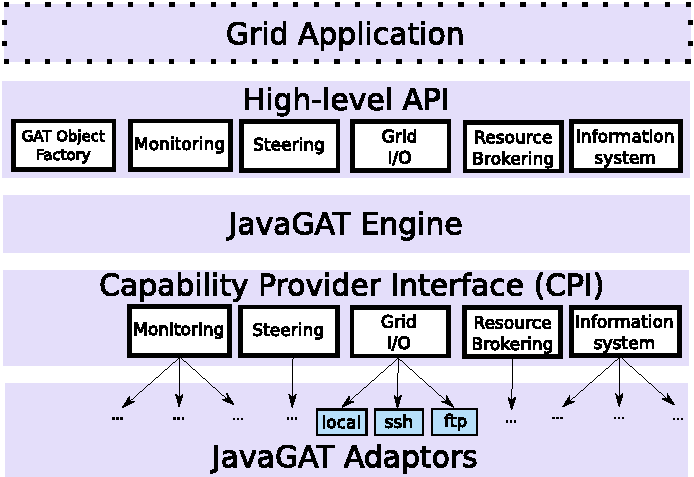
\includegraphics[clip,scale=0.5]{JavaGATFigure1}


\caption{\label{fig:JavaGAT structure}}

The structure of the JavaGAT implemententation, taken from \cite{JavaGAT}
\end{figure}


It consists out of different layers which all have its own responsibility.
The top layer is the API that serves as the interface to the user.
Below the API resides the engine. The engine is responsible for delegating
the API calls to the correct middleware. The Capability Provider Interface
is the layer which connects the engine to middleware specific software,
called adaptors. When the engine receives a request, i.e, to copy
a file, it selects the right adaptor with help from the CPI. The adaptor
then delegates the copy request to the actual middleware that copies
the file. 

Principles used from JavaGAT in the SAGA Java reference implementation
include the intelligent dispatching, nested exceptions and the adaptor
writing framework. The intelligent dispatching is the process where
the engine chooses the correct adaptor for the requested action and
the related preferences. Nested exceptions are special aggregations
of exceptions which come from the different adaptors. Adaptors might
raise exceptions when they fail at a certain action or do not implement
the requested action. All these exceptions are stored in a nested
exception and is only thrown to the grid application if every adaptor
failed at fulfilling the request. The adaptor writing framework makes
it easy for users to write or change adaptors with little effort.
This is an advantage because there are many middleware systems available
and they are changing often.

The Java reference implementation implements SAGA completely since
this is a requirement in the SAGA specification. There are still some
deviations from GFD.90, such as links and permissions. Java does not
have a notion of links and permissions so it is not possible to include
them. If methods relating to them are called, the implementation will
throw a \texttt{NotImplementedException}. The implemented Java language
binding also contains small extentions like file streams and using
RPC with objects instead of using Byte arrays.

Adaptors currently included with the Java reference implementation
are XMLRPC for RPC, Socket for streams, Gridsam for jobs, and Adaptors
from JavaGAT.


\subsubsection{C++ SAGA Reference Implementation}

Before the GFD.90 specification for SAGA was released a group at the
Louisiana State University \cite{LSU} started to build a C++ reference
implementation \cite{C++SAGA}. People from the group were also involved
in the SAGA design process and the developing of GAT and pioneered
in implementing a SAGA C++ implementation. This implementation works
in a similar way as the Java implementation as that it also includes
call routing through to the adaptors. It also features the probing
of multiple adaptors and the variable adaptor strategies. In addition,
it tries latency hiding strategies such as bulk optimalization and
automatic load distribution over multiple adaptors.

The implementation offers wrappers for C and Python but they are not
fully functional as they are in alpha stage. A Python language binding
is not available and the wrapper closely follows the syntax of the
underlying C++ layer. My Python language binding is specified top-down
from the SAGA specification, the wrapper is designed bottom-up from
the implementation.


\section{Python}

The Python language binding for SAGA is a specification of the classes
and methods in the programming language Python. In this section I
will explain parts of Python and how it influences the specification. 


\subsection{Introduction to Python}

Python was created in 1989 by Guido van Rossum who was working at
the Centrum voor Wiskunde en Informatica (CWI) in the Netherlands.
He worked on the programming language ABC, but needed some extra features.
Not wanting to fall back to C, he created his own language called
Python. 

Python is a high level interpreted scripting language and applications
do not have to be explicitly compiled. It is Object Oriented but also
borrows some features from functional languages. The Python interpreter
is written in C, sometimes called CPython, and is extensible by writing
your own modules or by writing special C modules for it. Because the
interpreter is written in C it is portable to platforms which support
the ANSI C compiler and scripts have to be written only once to be
run on many platforms. Some projects have rewritten the interpreter
in different programming languages to take advantage of the distict
features of the language. These projects include Jython for a Java
interpreter and IronPython for a C\# version. According to estimations
\cite{ProgLang}, the popularity of Python is around 5\%, after Java,
C, C++, VB and PHP. This rating is based on information from search
engines, engineers and companies world-wide. Together with Java, C++
and C, support for Python will give users enough choice for developing
applications using SAGA.


\subsection{Syntax Features}

Python has some features in its syntax which influenced the SAGA language
binding, and makes one to one copying of the SAGA specification not
as straight forward as it seems. In this section I will explain which
features those are.


\subsubsection{Dynamic Typing}

Python uses dynamic typing, which means that the type of a variable
is bound to the type of variable value, and can change regulary. In
static typing, the type is set when the variable is created and cannot
be changed afterwards. This gives new possibilities when dealing with
return values and parameter types. A commonly heard term is that Python
uses 'Duck Typing' ({}``If it looks like a duck and quacks like a
duck, it must be a duck.\char`\"{}). This means that calling a method
of an object is always possible. If it actually succeeds and does
not result in a runtime error depends on the object. In this context
it means that if you can call quack() and walk() on an object, the
type was probably Duck. If it gave a runtime error, the object was
definitly not a Duck. There are ways check the type of a variable,
like \texttt{type(), isinstance(), issubclass() or variable.\_\_class\_\_}
.


\subsubsection{Keywords and builtins}

Python has reserved keywords just like every programming language.
Most of these are are similar to other languages, but Python has some
specific ones which are also used in the SAGA specification. In the
\texttt{Permission} enum \texttt{Exec} and \texttt{None} are mentioned,
but both \texttt{exec} and \texttt{None} are reserved. Although Python
is case-sensitive, this gives problems when defining a consequent
namescheme.

Python also has some standard functions which are available. These
include functions like \texttt{list()}, \texttt{tuple()}, \texttt{dir()}
and \texttt{type()}. SAGA has some parameters names like which interfere
with the built in methods, such as \texttt{type} in the \texttt{Metric}
constructor.


\subsubsection{Methods}

Methods are defined in Python by using the \texttt{def} keyword followed
by the method name and the parameters in brackets. \texttt{def} defines
a method, but can also be used to overwrite the previously defined
method with the same name. This makes it impossible to do overloading,
defined as defining multiple methods with the same name but only differing
in parameter types. The same effect can still be archieved in Python
since the parameter type is not defined in the method declaration.
It does give difficulties if SAGA specification has overloaded methods
with completely different sets of parameter types.


\subsubsection*{Multiple Return Values}

Python also supports returning multiple variables from one method
call opposed to many other languages. This prevents using special
objects which hold more variables or special global variables. The
actual returned type is a special read-only list called a tuple, but
users can use multiple variables to automatically unpack the tuple
among the variables. See algorithm \ref{alg: multi ret values} for
an example.

%
\begin{algorithm}[h]
\texttt{def method():}

\texttt{~~~~variable1 = 'a String'}

\texttt{~~~~variable2 = 2}

\texttt{~~~~return variable1, variable2}~\\
 \texttt{}

\texttt{var1, var2 = method()}


\caption{\label{alg: multi ret values}Example of multiple return values in
Python}
\end{algorithm}


Since the variables are dynamically typed, the same method can return
multiple variables of different types. This feature is usable with
the \texttt{JobService.run\_job()} method since that method is specified
to return the job and three handles to the standard input, output
and error.


\subsubsection*{Default Parameter Values}

In the method declaration it is possible to specify default values
for parameters in the method definition. Not all parameters need default
values, but those that do specify them, need to be placed at the end.
Python needs this order to determine which given value in the method
call belongs to which parameter. See algorithm \ref{alg:Expl-defparameters}
for an example.

%
\begin{algorithm}[h]
\texttt{def write( buffer, size=3, offset=5):}

\texttt{~~~~pass}~\\


\texttt{write( buf )}

\texttt{write( buf, 3 )}

\texttt{write( buf, 3, 5 )}

\texttt{write( buf, offset=5 )}

\texttt{write( offset=5, size=3, buffer=buf)}


\caption{\label{alg:Expl-defparameters}Example of default parameters in Python.
Each \texttt{write()} call has exactly the same parameter values.
The \texttt{pass} statement does nothing, but leaving the method empty
will result in a syntax error. Python uses whitespace to define blocks
of code, also called suites.}
\end{algorithm}



\subsubsection*{Named Parameters}

When looking at the example of algorithm \ref{alg:Expl-defparameters}
you can notice that in the last two writes the parameter names are
explicitly mentioned. This explicit naming of the parameters allows
that when dealing with a large amount of defaulted parameters, you
can specify which parameters you want to change in the method call
instead of specifying all the parameters. An example is shown in algorithm
\ref{alg:Example-of-explicitly}.

%
\begin{algorithm}[h]
\texttt{def method( first=1, second=2, third=3, last = '4'):}

\texttt{~~~~pass}~\\


\texttt{method ( last = 'final')}


\caption{\label{alg:Example-of-explicitly}Example of explicitly naming the
parameters}
\end{algorithm}


To improve usability in the Python language binding, deceiding about
the order of the defaulted parameters is an interesting issue. A \texttt{File.read()}
call from the SAGA specification defined as \texttt{read(size='-1',
buffer=None)} has a different parameter order than a \texttt{File.write()}
call which is defined as \texttt{write( buffer, size='-1').} This
looks inconsistant, but is done because a data buffer is needed for
writing, but is optional for reading. The read data is returned as
a string. The amount of data read can be checked by doing a \texttt{len()}
call with the string as parameter, i.e: \texttt{len(returnedString)} 


\subsubsection*{Different Data Types}

Although Python supports many data types, it misses some types which
are standard in other languages and are mentioned in GFD.90. These
include enum, byte and char. Characters are just strings with a length
of one. The array package does have notion of a character to store
strings of length one, but there is no separate data type.

Python has no notion of an enum, but this can be solved in different
ways. First of all, a class can be constructed containing all the
values from the enum, such as the Flag enums in the SAGA specification.
Another solution is to use dictionaries, which have similarities with
hashtables in other languages. Dictionaries are commenly used in Python,
but their syntax is less straightforward than using simple objects
filled with variables.

The byte data type is missing from Python. This causes some confusion
how to specify and implement the mutable Buffer defined in SAGA. The
Buffer encapsulates a sequence of bytes to use in read and write operations
and is an essential part of SAGA. A possibility is to deny users to
use application managed buffers and use implementation managed buffers
only, but this would limit the use of Buffers in SAGA and exclude
a part of SAGA from the language binding. There is no standard to
use buffers and they are not available in Python. Users could write
their own buffer library, but it defeats the platform independent
principle. 

A solution was found in using arrays of chars. Arrays are guaranteed
to contain only the specified data type and if characters are read
or written they are immediatly visable to users. Problems may arise
if underlying implementations use different encodings for the characters,
like unicode, but that should be solved the programmers implementing
the language binding. Suggestions were made to me to completly remove
the buffers since they would be 'not Pythonesque' or 'Pythonic'%
\footnote{Although 'Pythonic' is an extremely vague term, Python programmers
generally assume there is only one correct way to do something. Other
solutions are not Pythonic.%
}.

Python also has support for numbers. Normally programmers will only
need an int. Int is internally implemented as a C long. If the int
overflows because two very large numbers are multiplied, Python will
automatically switch to a long. Longs can be arbitrarily long. Python
has no double but only a double-precision float. Shorts are also not
available in Python.


\subsubsection{Extending Python}


\subsubsection{Future versions of Python}


\subsection{Jython}


\subsection{Difference Jython - Python}


\section{Specification\label{sec:Specification}}


\subsection{All Modules Specified with Design Decisions}


\section{Implementation}

variable classes not write protected


\subsection{Previous work // Solutions Tested}


\subsection{Delegate Object}


\subsection{Convert Exception}


\subsection{Tasks}


\subsection{Inheritance}


\subsection{Get\_id()}


\subsection{All Modules Specified with Design Decisions}


\section{Testing}


\subsection{Test Environment}


\subsection{scripts}


\subsection{Bugs}


\subsection{Repository}


\section{Discussion}


\section{Future Work}


\subsection{Synchronize specification with LSU}


\subsection{Extending the API}

Extention packages


\subsection{Special Python operators}


\subsection{Updating Implementation with new Reference Implementations}


\section{List of Frequently Used Terms}

\begin{itemize}
\item API: Application Programming Interface. A set of variables, methods
and classes that is offered by an operating system or software library
to support requests made by computer programs. 
\item Grid: A collection of interconnected computers consisting of different
hardware, placed in different locations and belonging to different
organizations. 
\item Grid Aware: Applications which are grid aware are designed to run
on a grid and use the possibilities of the grid, such as distributing
workload between available nodes in the grid. 
\item Language Binding: An API in a specific programming language which
gives access to a library or service
\item Reference Implementation: First working software which implements
the functionality described by SAGA. New applications can link to
this software and call methods described in SAGA to use the grid.
\item SAGA: Simple API for Grid Applications 
\end{itemize}

\section{Conclusion}


\section{Bibliography}

\bibliographystyle{plain}
\addcontentsline{toc}{section}{\refname}\bibliography{Thesis}



\section{Acknowledgments}


\section{Appendix A: Installing and Running JySaga}


\section{Appendix B: Proof of a Higgs-boson}
\end{document}
